% This is a Basic Assignment Paper but with like Code and stuff allowed in it, there is also url, hyperlinks from contents included. 

\documentclass[11pt]{article}

% Preamble

\usepackage[margin=1in]{geometry}
\usepackage{amsfonts, amsmath, amssymb}
\usepackage{fancyhdr, float, graphicx}
\usepackage[utf8]{inputenc} % Required for inputting international characters
\usepackage[T1]{fontenc} % Output font encoding for international characters
\usepackage{fouriernc} % Use the New Century Schoolbook font
\usepackage[nottoc, notlot, notlof]{tocbibind}
\usepackage{listings}
\usepackage{xcolor}
\usepackage{blindtext}
\usepackage{hyperref}
\hypersetup{
    colorlinks=true,
    linkcolor=black,
    filecolor=magenta,      
    urlcolor=cyan,
    pdfpagemode=FullScreen,
    }

\definecolor{codegreen}{rgb}{0,0.6,0}
\definecolor{codegray}{rgb}{0.5,0.5,0.5}
\definecolor{codepurple}{rgb}{0.58,0,0.82}
\definecolor{backcolour}{rgb}{0.95,0.95,0.92}

\lstdefinestyle{mystyle}{
    backgroundcolor=\color{backcolour},   
    commentstyle=\color{codegreen},
    keywordstyle=\color{magenta},
    numberstyle=\tiny\color{codegray},
    stringstyle=\color{codepurple},
    basicstyle=\ttfamily\footnotesize,
    breakatwhitespace=false,         
    breaklines=true,                 
    captionpos=b,                    
    keepspaces=true,                 
    numbers=left,                    
    numbersep=5pt,                  
    showspaces=false,                
    showstringspaces=false,
    showtabs=false,                  
    tabsize=2
}

\lstset{style=mystyle}

% Header and Footer
\pagestyle{fancy}
\fancyhead{}
\fancyfoot{}
\fancyhead[L]{\textit{\Large{Advanced Data Structures - Assignment 5}}}
%\fancyhead[R]{\textit{something}}
\fancyfoot[C]{\thepage}
\renewcommand{\footrulewidth}{1pt}



% Other Doc Editing
% \parindent 0ex
%\renewcommand{\baselinestretch}{1.5}

\begin{document}

\begin{titlepage}
    \centering

    %---------------------------NAMES-------------------------------

    \huge\textsc{
        MIT World Peace University
    }\\

    \vspace{0.75\baselineskip} % space after Uni Name

    \LARGE{
        Advanced Data Structures\\
        Second Year B. Tech, Semester 4
    }

    \vfill % space after Sub Name

    %--------------------------TITLE-------------------------------

    \rule{\textwidth}{1.6pt}\vspace*{-\baselineskip}\vspace*{2pt}
    \rule{\textwidth}{0.6pt}
    \vspace{0.75\baselineskip} % Whitespace above the title



    \huge{\textsc{
            Implementation of a Graph and its Depth First and Breadth First Traversals
        }} \\



    \vspace{0.5\baselineskip} % Whitespace below the title
    \rule{\textwidth}{0.6pt}\vspace*{-\baselineskip}\vspace*{2.8pt}
    \rule{\textwidth}{1.6pt}

    \vspace{1\baselineskip} % Whitespace after the title block

    %--------------------------SUBTITLE --------------------------	

    \LARGE\textsc{
        Assignment No. 5
    } % Subtitle or further description
    \vfill

    %--------------------------AUTHOR-------------------------------

    Prepared By
    \vspace{0.5\baselineskip} % Whitespace before the editors

    \Large{
        Krishnaraj Thadesar \\
        Cyber Security and Forensics\\
        Batch A1, PA 20
    }


    \vspace{0.5\baselineskip} % Whitespace below the editor list
    \today

\end{titlepage}

\tableofcontents
\thispagestyle{empty}
\clearpage

\setcounter{page}{1}

\section{Objectives}
\begin{enumerate}
    \item \textit{To study data structure Graph and its representation using adjacency list}
    \item \textit{To study and implement recursive Depth First Traversal and use of stack data}
    \item \textit{structure for recursive Depth First Traversal}
    \item \textit{To study and implement Breadth First Traversal}
    \item \textit{To study how graph can be used to model real world problems}
\end{enumerate}

\section{Problem Statement}
Consider a friend's network on Facebook social web site. Model it as a graph to represent each
node as a user and a link to represent the friend relationship between them using adjacency list
representation and perform DFS and BFS traversals.

\section{Theory}

\subsection{Definition of Graph}

\textit{A graph is a non-linear data structure consisting of nodes and edges. The nodes are sometimes also referred to as vertices and the edges are lines or arcs that connect any two nodes in the graph. More formally a Graph can be defined as, a Graph consists of a finite set of vertices(or nodes) and set of Edges which connect a pair of nodes.}

\begin{figure}[H]
    \centering
    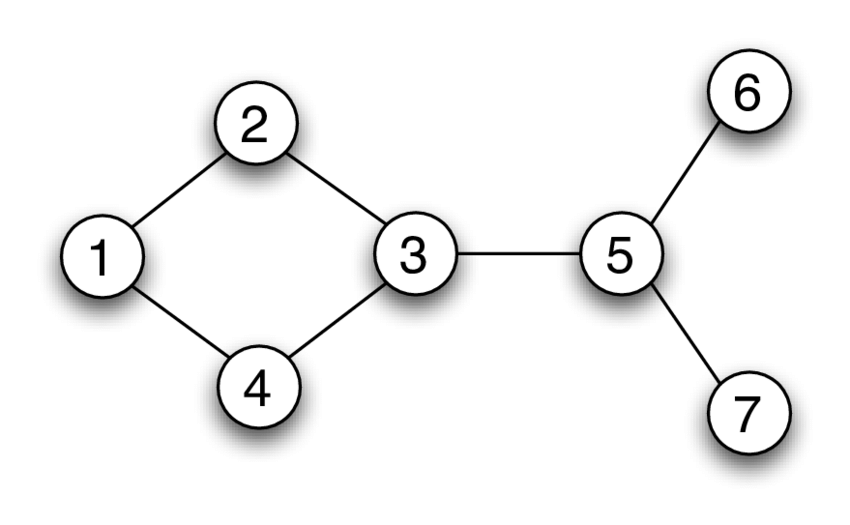
\includegraphics[width=.45\textwidth]{figures/undirected graph.png}
    \caption{Graph}
\end{figure}

\subsection{Types of Graph}
\subsubsection{Directed Graph}
\textit{A directed graph, also known as a digraph, is a type of graph in which edges have a direction. It represents relationships between objects that have a cause-and-effect relationship, such as a food chain. For example, a food chain of lions, zebras, and grass can be represented as a directed graph where the edge points from zebras to lions, lions to grass, and grass to zebras.}

\begin{figure}[H]
    \centering
    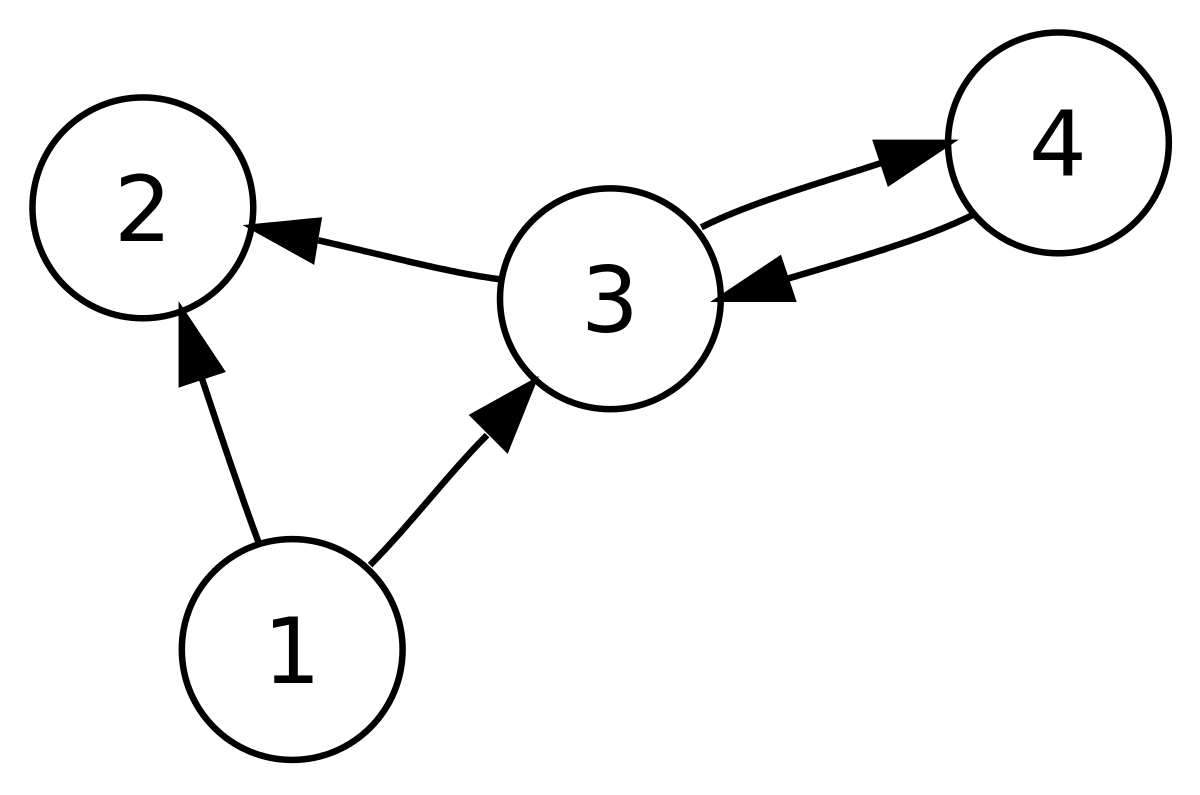
\includegraphics[width=.45\textwidth]{figures/directed graph.png}
    \caption{Directed Graph}
\end{figure}

\subsubsection{Undirected Graph}

\textit{An undirected graph is a type of graph in which edges have no direction. It represents relationships between objects that have a symmetric relationship, such as social networks. For example, a social network of friends can be represented as an undirected graph where each node represents a person, and an edge connects two people if they are friends.}

\begin{figure}[H]
    \centering
    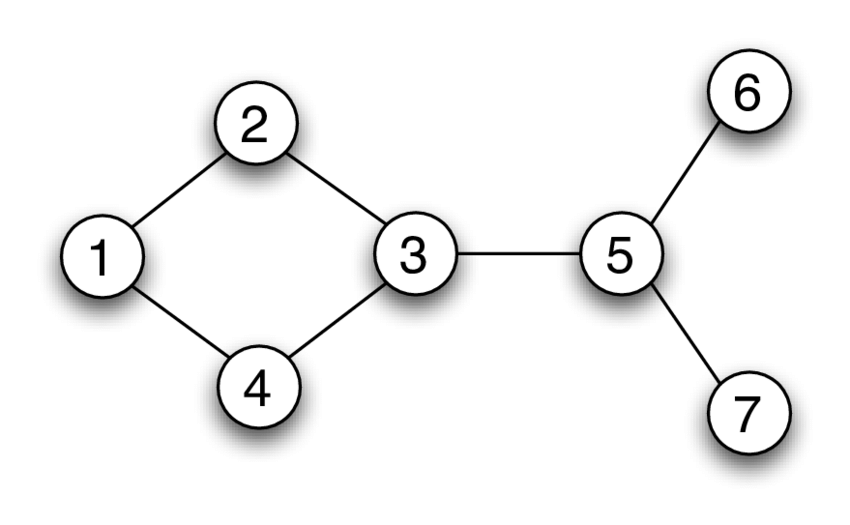
\includegraphics[width=.45\textwidth]{figures/undirected graph.png}
    \caption{Undirected Graph}
\end{figure}

\subsubsection{Weighted Graph}

\textit{A weighted graph is a type of graph in which edges have a numerical value. It is used to represent relationships between objects where the relationship has a quantity associated with it, such as distances between cities. For example, a map of cities can be represented as a weighted graph where the nodes represent cities and the edges represent distances between them.}

\begin{figure}[H]
    \centering
    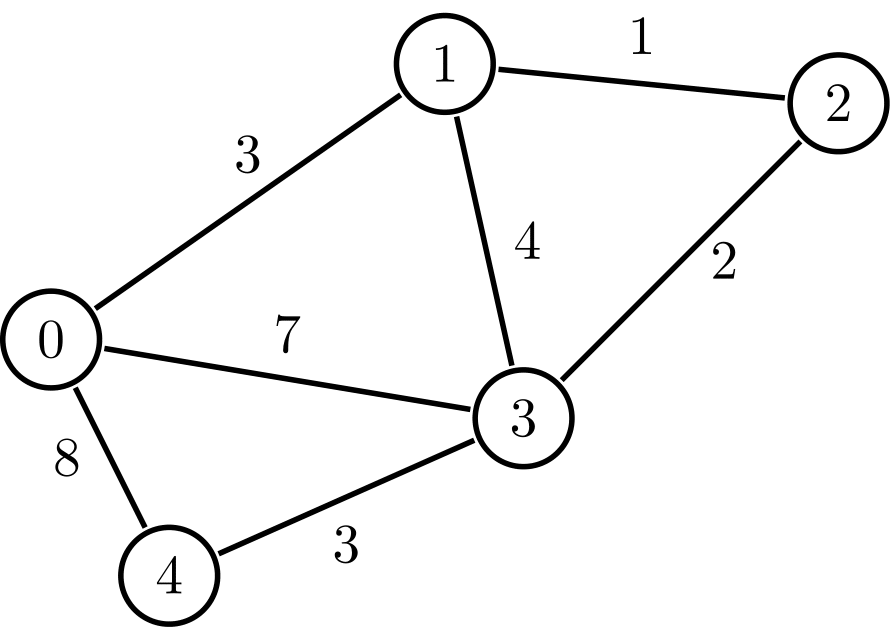
\includegraphics[width=.45\textwidth]{figures/weighted graph.png}
    \caption{Weighted Graph}
\end{figure}


\subsubsection{Bipartite Graph}

\textit{A bipartite graph is a type of graph in which the nodes can be divided into two disjoint sets, such that each edge connects a node in one set to a node in the other set. It is used to represent relationships between two different sets of objects, such as employers and employees. For example, a company can be represented as a bipartite graph where one set of nodes represents employers and the other set represents employees, and an edge connects an employer to an employee if the employer employs the employee.}

\begin{figure}[H]
    \centering
    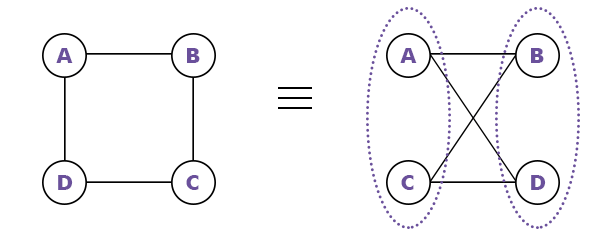
\includegraphics[width=.45\textwidth]{figures/bipartite graph.png}
    \caption{Bipartite Graph}
\end{figure}


%  Representation of graph using adjacency list with one example and diagram.
%  Graph Traversals DFT and BFT with example and diagrams


\section{Platform}
\textbf{\textbf{Operating System}}: Arch Linux x86-64 \\
\textbf{\textbf{IDEs or Text Editors Used}}: Visual Studio Code\\
\textbf{\textbf{Compilers} }: g++ and gcc on linux for C++\\

\section{Input}
\begin{enumerate}
    \item Input at least 5 nodes.
    \item Display DFT (recursive and non recursive) and BFT
\end{enumerate}

\section{Output}
\begin{enumerate}
    \item The traversal of the Threaded binary tree in different ways.
\end{enumerate}

\section{Test Conditions}
\begin{enumerate}
    \item Input at least 10 nodes.
    \item Display all traversals of binary tree with 10 nodes.(recursive and nonrecursive)
\end{enumerate}

\section{Pseudo Code}
\subsection{Creation of the Graph}
\begin{lstlisting}[language=C++]
	//Pseudo Code for Creation of Threaded Binary Tree

\end{lstlisting}
\subsection{Depth First Search (Recursive)}
\begin{lstlisting}[language=C++]
    
\end{lstlisting}

\subsection{Depth First Search (Non Recursive)}
\begin{lstlisting}[language=C++]
    
\end{lstlisting}

\subsection{Breadth First Search}
\begin{lstlisting}[language=C++]
\end{lstlisting}

\section{Time Complexity}

\subsection{Creation of Threaded Binary Tree}
\begin{itemize}
    \item \textbf{Time Complexity:} \[O(V^2)\] for adjacency matrix representation\\
    where V is the number of vertices in the graph, and E is the number of edges in the graph.
    \item \textbf{Time Complexity:} \[O(E)\] for adjacency list representation\\
    where V is the number of vertices in the graph
    \item \textbf{Space Complexity:} \[O(V^2)\] for V being the number of vertices in the graph.
\end{itemize}

\subsection{Recursive Depth First Traversal}

\begin{itemize}
    \item \textbf{Time Complexity:} \[O(V+E)\] for V being the number of vertices in the graph and E being the number of edges in the graph.
    \item \textbf{Space Complexity:} \[O(V)\] for V being the number of vertices in the graph.
\end{itemize}

\subsection{Non Recursive Depth First Traversal}

\begin{itemize}
    \item \textbf{Time Complexity:} \[O(V+E)\] for V being the number of vertices in the graph and E being the number of edges in the graph.
    \item \textbf{Space Complexity:} \[O(V)\] for V being the number of vertices in the graph.
\end{itemize}


\subsection{Breadth First Traversal}

\begin{itemize}
    \item \textbf{Time Complexity:} \[O(V+E)\] for V being the number of vertices in the graph and E being the number of edges in the graph.
    \item \textbf{Space Complexity:} \[O(V)\] for V being the number of vertices in the graph.
\end{itemize}


\section{Code}

\subsection{Program}
\lstinputlisting[language=C++]{../Programs/Assignment_5.cpp}

\subsection{Input and Output}
\lstinputlisting[]{../Programs/Assignment_5_output.txt}

\section{Conclusion}
Thus, we have represented graph using adjacency list and performed DFT and BFT.

\clearpage

\section{FAQ}
\begin{enumerate}
\item \textbf{Explain two applications of graph.}\\

Graphs have numerous applications in various fields such as computer science, social sciences, biology, transportation, and more. Here are two examples of applications of graphs:
\begin{itemize}
    \item \textbf{Social Networks}: Social networks such as Facebook, Twitter, and LinkedIn can be represented as graphs, where each user is a node, and the relationship between them (friendship, follow, connection, etc.) is an edge. Graph algorithms can be used to analyze and understand social networks, such as identifying clusters of friends, finding influential users, detecting fake accounts or spam, and predicting trends or user behavior. For example, graph analysis can help social networks to recommend new friends, suggest content to users, or optimize their algorithms to improve user engagement and retention.

    \begin{figure}[H]
        \centering
        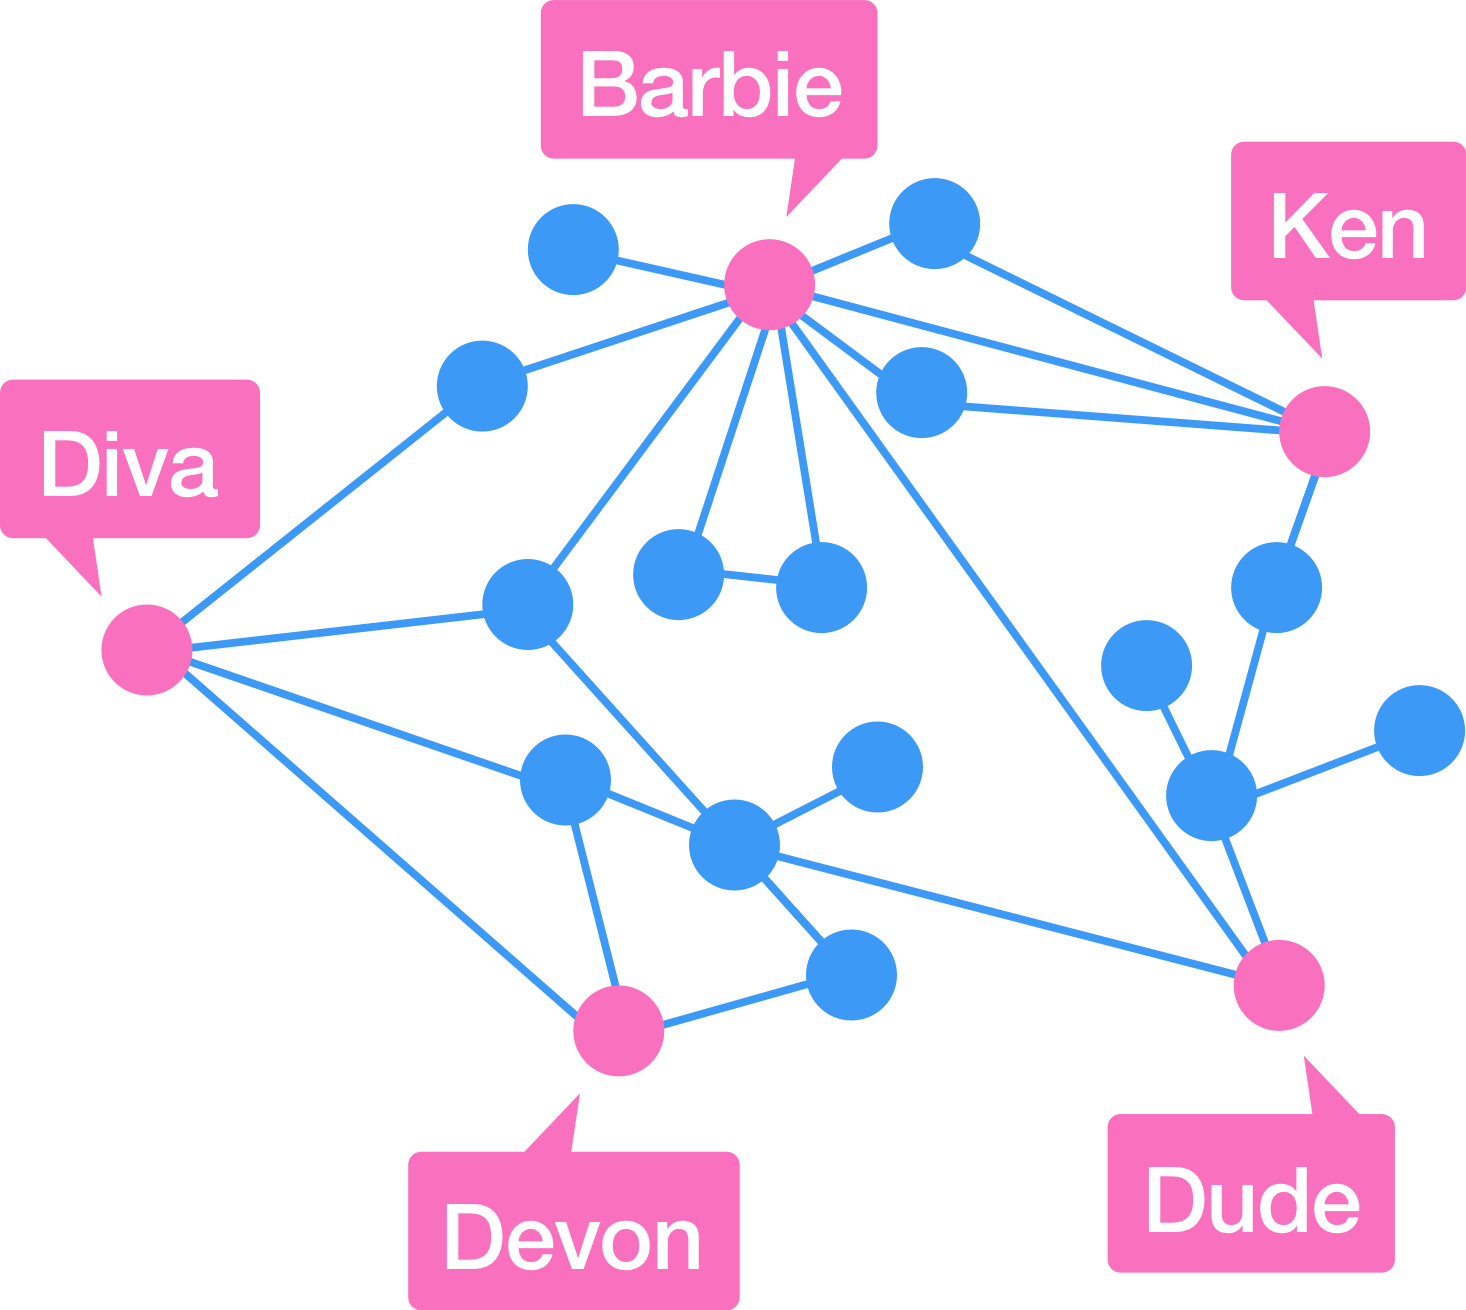
\includegraphics[width=.45\textwidth]{figures/social_media.png}
        \caption{Graph as a Representation for Social Media}
    \end{figure}
    
    \item \textbf{Shortest Path Algorithms}: Graphs can be used to model transportation networks such as roads, railways, and flights, where each city or location is a node, and the roads or flights connecting them are edges. Shortest path algorithms such as Dijkstra's algorithm and the A* algorithm can be used to find the shortest path or the fastest route between two locations, taking into account factors such as distance, time, traffic, or cost. These algorithms are widely used in navigation systems, logistics, and transportation planning, and can help optimize the routing and scheduling of vehicles, goods, or passengers, leading to cost savings and improved efficiency.
    
    \begin{figure}[H]
        \centering
        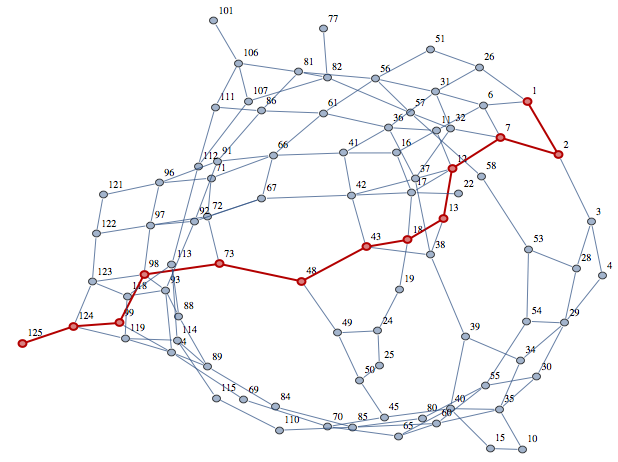
\includegraphics[width=.85\textwidth]{figures/shortest path.png}
        \caption{The Shortest Path Problem represented and solved using a Graph}
    \end{figure}
\end{itemize}


\item \textbf{Explain advantages of adjacency list over adjacency matrix.}\\

The adjacency list representation of a graph has the following advantages over an adjacency matrix representation:
\begin{itemize}
    \item \textbf{Space Efficient}: The adjacency list representation is more space efficient than the adjacency matrix representation. This is because the adjacency matrix representation of a graph with V vertices and E edges requires O($V^2$) space, while the adjacency list representation requires O(V+E) space.
    \item \textbf{Faster Adjacent Edge Lookups}: The adjacency list representation allows for faster lookups of adjacent edges of a vertex than the adjacency matrix representation. In the adjacency matrix representation, to find the adjacent edges of a vertex, we have to scan through the entire row of the vertex. In the adjacency list representation, we can simply traverse the linked list of the vertex to find its adjacent edges.
    \item \textbf{Faster Degree Lookups}: The adjacency list representation allows for faster lookups of the degree of a vertex than the adjacency matrix representation. In the adjacency matrix representation, to find the degree of a vertex, we have to scan through the entire row of the vertex. In the adjacency list representation, we can simply traverse the linked list of the vertex to find its degree.
\end{itemize}

\item \textbf{Why transversal in graph is different than traversal in tree}\\

\begin{itemize}
    \item \textbf{Graphs can have cycles}: Unlike trees, graphs can contain cycles, which means that a node can be visited multiple times through different paths. This makes traversal more complex, as we need to keep track of the visited nodes to avoid infinite loops or redundant computations. In trees, on the other hand, there are no cycles, so each node is visited exactly once during traversal.

    \item \textbf{Graphs can be disconnected}: Graphs can have disconnected components, which means that some nodes may not be reachable from others. This means that traversal of a graph needs to handle the possibility of having multiple disconnected components, and ensure that all components are visited. In contrast, trees are always connected, so there is no need to worry about disconnected components.
    
    \item \textbf{Graphs can be directed or undirected}: Graphs can be either directed (where edges have a direction) or undirected (where edges have no direction), which affects how traversal algorithms operate. For example, in a directed graph, traversal algorithms need to take into account the direction of edges to avoid going back to already-visited nodes, while in an undirected graph, traversal can simply use a marking mechanism to track visited nodes.
\end{itemize}

\end{enumerate}

\end{document}